\documentclass[a4paper,12pt]{article}

\usepackage{cmap}					% поиск в PDF
\usepackage{mathtext} 				% русские буквы в формулах
\usepackage[T2A]{fontenc}			% кодировка
\usepackage[utf8]{inputenc}			% кодировка исходного текста
\usepackage[english,russian]{babel}	% локализация и переносы

\usepackage{amsfonts,amssymb,amsthm,mathtools} % AMS
\usepackage{amsmath}
\usepackage{icomma} % "Умная" запятая

\usepackage{euscript}
\usepackage{mathrsfs}

\newcommand*{\hm}[1]{#1\nobreak\discretionary{}
{\hbox{$\mathsurround=0pt #1$}}{}}

\usepackage{graphicx}  % Для вставки рисунков

\usepackage{caption}
\captionsetup{labelsep=period}

\usepackage{wrapfig} % Обтекание рисунков и таблиц текстом



\begin{document}

Пусть рис.\ref{fig:21} представляет положения Солнца $S$, Земли $T$ и Луны $L$, и пусть $\Theta$ есть центр тяжести Земли и Луны. Делаем следующие обозначения:
\begin{table}[!h]
  \begin{center}
    \begin{tabular}{cccccccc}
      Масса & Солнца & . & . & . & . & . & S \\
      >> & Земли & . & . & . & . & . & T \\
      >> & Луны & . & . & . & . & . & L
    \end{tabular}
  \end{center}
  \caption{Массы}\label{tbl:masses}
\end{table}

Расстояние
\[ S\Theta = \rho; \: ST = \rho_1; \: SL = \rho_2; \: TL = r \]

тогда будет:
\begin{equation}
	\begin{aligned}
		T\Theta = r_1 = \frac{L}{T+L} \cdot r \\
		L\Theta = r_2 = \frac{T}{T+L} \cdot r
	\end{aligned}
\end{equation}

Составим теперь выражения ускорений, которые эти тела сообщают друг другу.

\begin{wrapfigure}{l}{0.5\linewidth}
  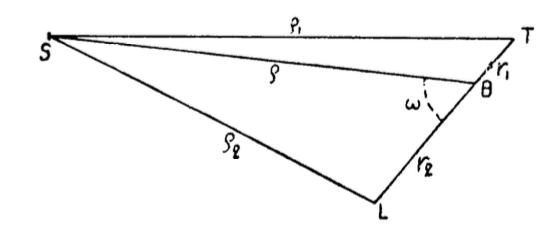
\includegraphics[width=0.9\linewidth,keepaspectratio]{21.png}
  \caption{}\label{fig:21}
\end{wrapfigure}

Солнце S сообщает ускорения:
\begin{equation*}
	\begin{aligned}
      Земле: && f \cdot \frac{S}{\rho_1 ^2} && \text{по направлению} && TS \\
      Луне: && f \cdot \frac{S}{\rho_2 ^2} && >> && LS
  \end{aligned}
\end{equation*}

вследствие чего точка $\Theta$ имеет ускорения:
\begin{equation*}
  \begin{aligned}
    \frac{T}{T+L} \cdot f \cdot \frac{S}{\rho_1 ^2} && \text{по направлению параллельному} && TS \\
    \frac{L}{T+L} \cdot f \cdot \frac{S}{\rho_2 ^2} && >> && LS
  \end{aligned}
\end{equation*}

Ускорения Солнца, происходящие от притяжения Земли и Луны, соответственно, суть:
\begin{equation*}
  \begin{aligned}
      f \cdot \frac{T}{\rho_1 ^2} && \text{по направлению} && ST \\
      f \cdot \frac{L}{\rho_2 ^2} && >> && SL
  \end{aligned}
\end{equation*}

поэтому ускорения точки $\Theta$ относительно точки S будут:
\begin{equation*}
  \begin{aligned}
      w_1 = f \cdot \frac{S+T+L}{T+L} \cdot \frac{T}{\rho_1 ^2} && \text{по направлению параллельно} && TS \\
      w_2 = f \cdot \frac{S+T+L}{T+L} \cdot \frac{L}{\rho_2 ^2} && >> && LS
  \end{aligned}
\end{equation*}

Разлагая эти ускорения, соответственно, по направлениям $\Theta S$ и $\Theta L$, получим, как легко видеть из подобия показанных на рис.\ref{fig:22} и \ref{fig:23} треугольников:
\begin{equation*}
  \begin{aligned}
      w_1 ' = w_1 \cdot \frac{\rho}{\rho_1} && \text{по направлению} && \Theta S \\
      w_1 '' = w_1 \cdot \frac{r_1}{\rho_1} && >> && \Theta L \\
      w_2 ' = w_2 \cdot \frac{\rho}{\rho_2} && >> && \Theta S \\
      w_2 '' = w_2 \cdot \frac{r_2}{\rho_2} && >> && L \Theta
  \end{aligned}
\end{equation*}

\begin{figure}[!h]
  \begin{center}
    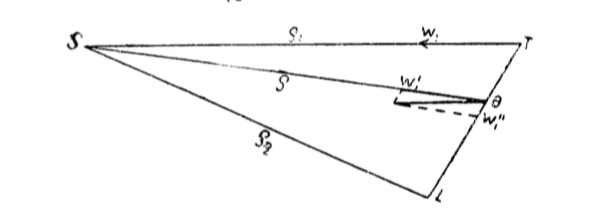
\includegraphics[width=0.7\linewidth, keepaspectratio]{22.png}
    \caption{}\label{fig:22}
  \end{center}
\end{figure}

получим для ускорений точки $\Theta$ слагающие:
\begin{equation*}
	\begin{aligned}
		W_1 = w_1 ' + w_2 ' = f \cdot \frac{S+T+L}{T+L} \cdot \left[ T \cdot \frac{\rho}{\rho_1 ^3} + L \cdot \frac{\rho}{\rho_2 ^3} \right] \, по \, \Theta S \\
		W_2 = w_1 '' - w_2 '' = f \cdot \frac{S+T+L}{T+L} \cdot \left[ T \cdot \frac{r_1}{\rho_1 ^3} - L \cdot \frac{r_2}{\rho_2 ^3} \right] \, по \, \Theta L
	\end{aligned}
\end{equation*}

\begin{figure}[!h]
  \begin{center}
    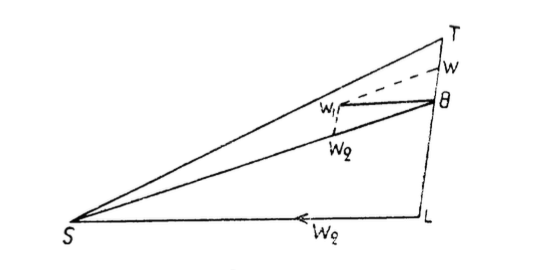
\includegraphics[width=0.7\linewidth, keepaspectratio]{23.png}
    \caption{}\label{fig:23}
  \end{center}
\end{figure}

Заменив $r_1$ и $r_2$ их выражениями (1), имеем:
\begin{equation*}
	\begin{aligned}
		W_1 = f \cdot \frac{S+T+L}{T+L} \cdot \rho \cdot \left[ \frac{T}{\rho_1 ^3} + \frac{T}{\rho_2 ^3} \right] \, \text{по направлению $\Theta$S} \\
		W_2 = f \cdot \frac{S+T+L}{(T+L)^2} \cdot T \cdot L \cdot r \left[\frac{1}{\rho_1 ^3} - \frac{1}{\rho_2 ^3} \right] \, \text{по направлению $\Theta$L}
	\end{aligned}
\end{equation*}

Но
\begin{equation*}
	\begin{aligned}
      \rho_1 ^2 = \rho^2 + 2\rho \cdot \frac{L}{T+L} \cdot r \cos \omega + \left( \frac{L}{T+L} \cdot r \right) ^2 \\
      \rho_2 ^2 = \rho^2 - 2\rho \cdot \frac{L}{T+L} \cdot r \cos \omega + \left( \frac{T}{T+L} \cdot r \right) ^2
	\end{aligned}
\end{equation*}

следовательно:
\begin{equation*}
	\begin{aligned}
      \frac{1}{\rho_1 ^3} = \frac{1}{\rho^3} \left[ 1 + 3 \frac{L}{T+L} \cos \omega + \left( \frac{L}{T+L} \cdot r \right) ^2 \left(-\frac{3}{2} + \frac{15}{2} \cos^2 \omega \right) + \dots \right] \\
      \frac{1}{\rho_2 ^3} = \frac{1}{\rho^3} \left[ 1 + 3 \frac{T}{T+L} \cos \omega + \left( \frac{T}{T+L} \cdot r \right) ^2 \left(-\frac{3}{2} + \frac{15}{2} \cos^2 \omega \right) + \dots \right]
	\end{aligned}
\end{equation*}

Подставляя эти выражения, имеем:
\begin{equation*}
	\begin{aligned}
      W_1 = f \cdot \frac{S+T+L}{\rho^2} \left[ 1 + \frac{T \cdot L}{(T+L)^2} \cdot \frac{r^2}{\rho^2} \left( -\frac{3}{2} + \frac{15}{2} \cos^2 \omega \right) + \dots \right] \\
      W_2 = f \cdot \frac{S+T+L}{\rho^2} \left[ -3 \cdot \frac{T \cdot L}{(T+L)^2} \cdot \frac{r^2}{\rho^2} \cos \omega + \dots \right]
	\end{aligned}
\end{equation*}

Но отношения
\[ \frac{L}{T+L} \approx \frac{1}{80}; \; \frac{r}{\rho} \approx \frac{1}{400}; \; \left( \frac{r}{\rho} \right) ^2 = \frac{1}{160000}\]

поэтому будет
\[ \frac{T \cdot L}{(T+L)^2} \cdot \frac{r^2}{\rho ^2} \approx \frac{1}{12800000} \]

и члены, содержащие этот множительн, могут быть отброшены, так что будет:
\begin{equation*}
	\begin{aligned}
		W_1 = f \cdot \frac{S+T+L}{\rho^2} \, \text{по направлению $\Theta$S} \\
		W_2 = 0 \, \text{по направлению $\Theta$L}
	\end{aligned}
\end{equation*}

Отсюда следует, что точка $\Theta$ движется вокруг Солнца по эллиптической орбите по законам Кеплера.

Рассмотрим теперь ускорение Луны по отношению к Земле, для чего к ускорениям, сообщаемым Луне Солнцем и Землею, надо присовокупить ускорение, равное и противоположное ускорению Земли, происходящему от действия Солнца и Луны.
Поступив подобно предыдущему, получим:
\begin{equation*}
	\begin{aligned}
		f \cdot \frac{T+L}{r^2} + f \cdot S \left[ \frac{r_2}{\rho_2 ^3} + \frac{r_1}{\rho_1 ^3} \right] \text{по направлению L$\Theta$} \\
		f \cdot S \cdot \rho \left[ \frac{1}{\rho_2 ^3} - \frac{1}{\rho_1 ^3} \right] \text{параллельно $\Theta$S}
	\end{aligned}
\end{equation*}

положим:
\[ T+L = \mu; \; S = M\]

\listoffigures

\listoftables

\end{document}
